\documentclass{article}
\usepackage[utf8]{inputenc}
\usepackage[english]{babel}
\usepackage[]{amsthm} 
\usepackage[]{amssymb} 
\usepackage{amsmath}
\DeclareMathOperator{\domain}{dom}
\usepackage{graphicx}
\usepackage{hyperref}
\usepackage{comment}
\usepackage[dvipsnames]{xcolor}
\usepackage[thinc]{esdiff}
\usepackage{tcolorbox}
\usepackage{cancel}
\usepackage{graphicx}
\usepackage{float}
\graphicspath{ {./HW2_images/} }
\newtheorem*{theorem}{Theorem}
\newenvironment{solution}
  {\renewcommand\qedsymbol{$\blacksquare$}\begin{proof}[Solution]}
  {\end{proof}}

\newenvironment{claim}[1]{\par\noindent\underline{Claim:}\space#1}{}
\newenvironment{claimproof}[1]{\par\noindent\underline{Proof:}\space#1}{}
\DeclareMathOperator{\interior}{int}


\title{Optimization Algorithms: HW2}
\author{Lo Chun, Chou \\ R13922136}
\date\today

\begin{document}
\setlength{\parindent}{0pt}
\maketitle 

\tcbset{
    greenbox/.style={
        colback=SpringGreen!20,
        colframe=SpringGreen!80,
        coltitle=black,
        sharp corners
    },
    bluebox/.style={
        colback=SkyBlue!20,
        colframe=SkyBlue!80,
        coltitle=black,
        sharp corners
    },
    yellowbox/.style={
        colback=yellow!10,
        colframe=yellow!80,
        coltitle=black,
        sharp corners
    }
}

\section*{1}

We're given the following problem:

\begin{align*}
    x_{\star} \in \arg\min_{x \in \Delta_d} f(x), \qquad f(x) = -\sum_{i=1}^n w_i \log \langle a_i, x \rangle
\end{align*}

where:

\begin{enumerate}
    \item 
    \begin{align*}
        x \in \Delta_d = \{ x \in \mathbb{R}^d \mid x[i] \geq 0, \sum_{i=1}^d x[i] = 1 \} \ (\text{probabilit`y simplex})
    \end{align*}
    \item 
    \begin{align*}
        w_i \in \mathbb{R}, \ w_i > 0, \ \sum_{i=1}^n w_i = 1
    \end{align*}
    \item 
    \begin{align*}
        &a_i \in \mathbb{R}^d, \ 
        a_i =
        \begin{bmatrix}
            a_i[1] \\
            a_i[2] \\
            \vdots \\
            a_i[d]
        \end{bmatrix}, \\ 
        &a_i[j] \geq 0 \ \forall i = 1, \dots, n, \ j = 1, \dots, d \\
        &a_i \neq 0 \ \forall i = 1, \dots, n
    \end{align*}
\end{enumerate}

We're asked to show that:

$f$ is $1$-smooth relative to the log-barrier, which is defined as:

\begin{align*}
    h(x) = -\sum_{i=1}^d \log x[i]
\end{align*}

\begin{solution}
%     By lecture slide 4, p.13, we have the definition of relative smoothness:
    
%     \begin{tcolorbox}[bluebox]
%         A function $f$ is $L$-smooth relative to a convex function $h$ for some $L > 0$ if:
%         \begin{align*}
%             f(y) \leq f(x) + \langle \nabla f(x), y - x \rangle + L D_h(y, x)
%         \end{align*}
%     \end{tcolorbox}
% \end{solution}

% Therefore, we need to prove that the following condition holds:

% \begin{align*}
%     -\sum_{i=1}^n w_i \log \langle a_i, y \rangle 
%     \leq -\sum_{i=1}^n w_i \log \langle a_i, x \rangle + \langle \nabla f(x), y - x \rangle + L \{ h(y) - \left[h(x) + \langle \nabla h(x), (y - x) \rangle \right]\}
% \end{align*}

By the following proposition
\footnote{\textit{Relative Smooth Convex Optimization by First-Order Methods, and Applications}, MIT Lecture Notes, available at: \url{https://dspace.mit.edu/bitstream/handle/1721.1/120867/16m1099546.pdf}, accessed: May.~9, 2025, p.~336.}:
\begin{figure}[H]
    \centering
    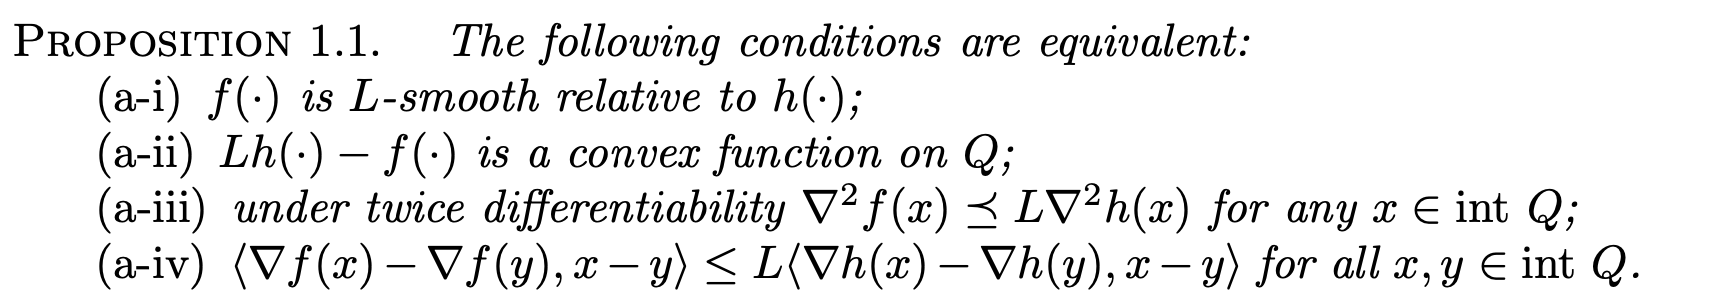
\includegraphics[width = 0.8\textwidth]{proposition_1.1}
\end{figure}
\bigskip

we could prove the required condition (which is (a-i), with $L = 1$) 
by proving its equivalent condition (a-iii, with $L = 1$).
\bigskip

First calculate $\nabla f(x)$:

\begin{align*}
    \nabla f(x) 
    &= \frac{d}{dx} \left( -\sum_{i=1}^n w_i \log \langle a_i, x \rangle \right) \\
    &= -\sum_{i=1}^n w_i \cdot \frac{d}{dx} \left( \log \langle a_i, x \rangle \right) \\
    &= -\sum_{i=1}^n w_i \cdot \left(\frac{a_i}{\langle a_i, x \rangle}\right) \\
    &= -\sum_{i=1}^n w_i \frac{a_i}{\langle a_i, x \rangle}
\end{align*}

Then the Hessian of $f$ is:

\begin{align*}
    \nabla^2 f(x) 
    &= \frac{d}{dx} \left( -\sum_{i=1}^n w_i \frac{a_i}{\langle a_i, x \rangle} \right) \\
    &= -\sum_{i=1}^n w_i \cdot \frac{d}{dx} \left( \frac{a_i}{\langle a_i, x \rangle} \right) \\
    &= -\sum_{i=1}^n w_i \cdot \left( \frac{a_i }{\langle a_i, x \rangle^2} a_i^T\right) \\
\end{align*}

Expanding the expression and writing in another form, we have:

\begin{align*}
    \nabla^2 f(x) 
    &= -\sum_{i=1}^n \frac{w_i}{\langle a_i, x \rangle^2} a_i a_i^T \tag{1}
\end{align*}

Then we shall do the same to $h(x)$

\begin{align*}
    \nabla h(x) 
    &= \frac{d}{dx} \left( -\sum_{i=1}^d \log x[i] \right) \\
    &= 
    \begin{bmatrix}
        -\frac{1}{x[1]} \\
        -\frac{1}{x[2]} \\
        \vdots \\
        -\frac{1}{x[d]}
    \end{bmatrix}
\end{align*}

Then $\nabla^2 h(x)$ is:

\begin{align*}
    \nabla^2 h(x) 
    &= \nabla 
    \begin{bmatrix}
        -\frac{1}{x[1]} \\
        -\frac{1}{x[2]} \\
        \vdots \\
        -\frac{1}{x[d]}
    \end{bmatrix} \\
    &= 
    \begin{bmatrix}
        &\frac{d}{dx[1]} \left( -\frac{1}{x[1]} \right) &\frac{d}{dx[2]} \left( -\frac{1}{x[1]} \right) &\cdots &\frac{d}{dx[d]} \left( -\frac{1}{x[1]} \right) \\
        &\frac{d}{dx[1]} \left( -\frac{1}{x[2]} \right) &\frac{d}{dx[2]} \left( -\frac{1}{x[2]} \right) &\cdots &\frac{d}{dx[d]} \left( -\frac{1}{x[2]} \right) \\
        &\vdots & & \ddots & \vdots \\
        &\frac{d}{dx[1]} \left( -\frac{1}{x[d]} \right) &\frac{d}{dx[2]} \left( -\frac{1}{x[d]} \right) &\cdots &\frac{d}{dx[d]} \left( -\frac{1}{x[d]} \right)
    \end{bmatrix} \\
    &=
    \begin{bmatrix}
        \frac{1}{x[1]^2} & 0 & \cdots & 0 \\
        0 & \frac{1}{x[2]^2} & \cdots & 0 \\
        \vdots & & \ddots & \vdots \\
        0 & 0 & \cdots & \frac{1}{x[d]^2}
    \end{bmatrix} \tag{2}
\end{align*}

Observe $\nabla^2 f(x)$ in $(1)$, since we're given $w_i > 0$, $x \in \Delta_d$, $a_i \neq 0$, 
and with proposition (a-iii) only requires dealing with $\interior \Delta_d$,
we can guarantee $x[i] > 0$, 
so the scalar $\frac{w_i}{\langle a_i, x \rangle^2} > 0$.
\bigskip

Also, we knew that for any $a_i \neq 0$, $a_i a_i^T$ is positive semidefinite,
thus, each term in the summation is positive semidefinite, 
by summing up the $n$ terms and adding a negative sign,
we have $\nabla^2 f(x) \preceq 0$ as follows:

\begin{align*}
    \nabla^2 f(x) 
    = -\sum_{i=1}^n \frac{w_i}{\langle a_i, x \rangle^2} a_i a_i^T \preceq 0
\end{align*}



% We then first show that $\nabla^2 f(x)$ is symmetric, and $\nabla^2 h(x)$ is positive definite,
% in order to use the following generalized Rayleigh quotient to prove that $\nabla^2 f(x) \preceq L \nabla^2 h(x)$:

% \begin{figure}[H]
%     \centering
%     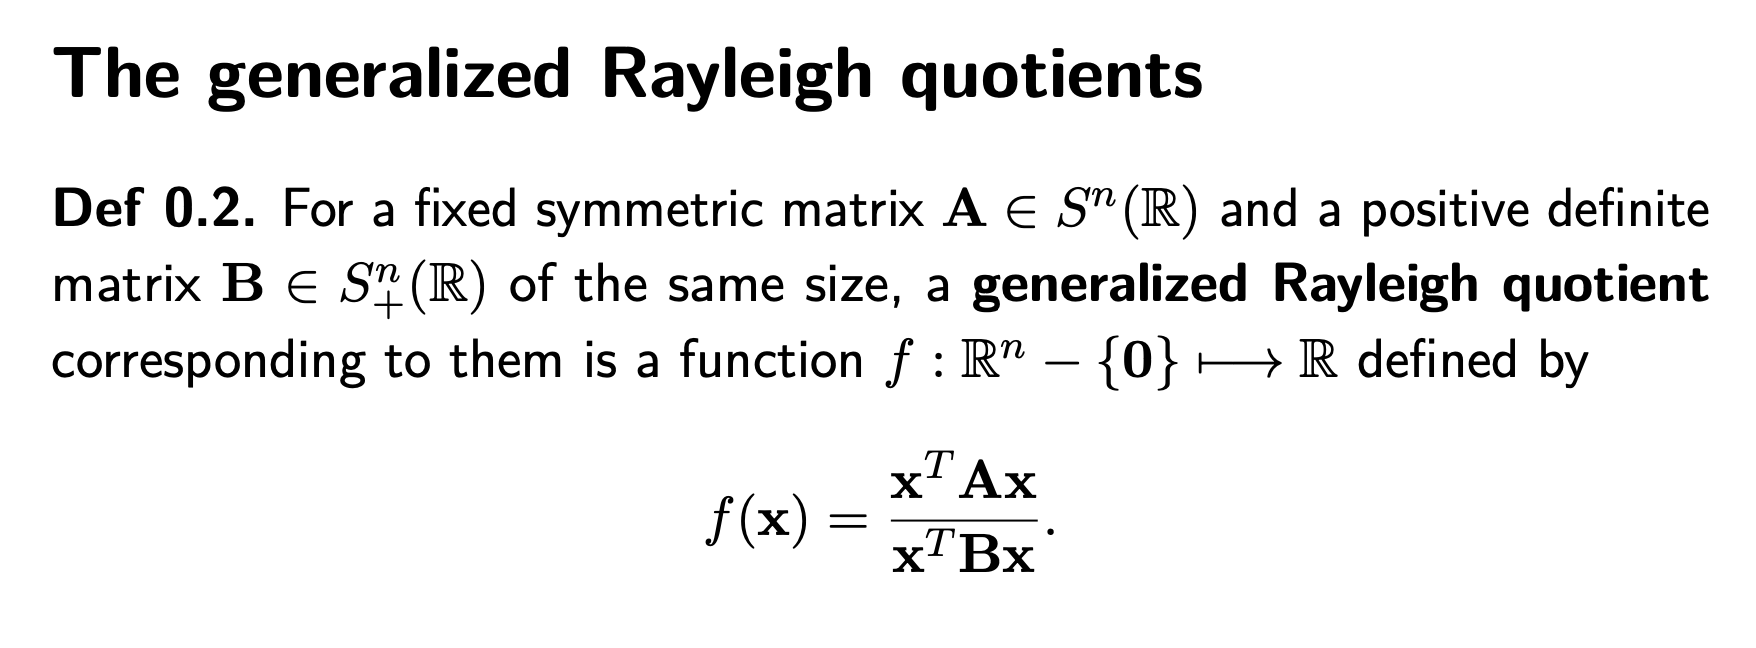
\includegraphics[width = 0.8\textwidth]{generalized_rayleigh_quotients.png}
% \end{figure}

% By our previous calculation, we have:

% \begin{align*}
%     \nabla^2 f(x) = -\sum_{i=1}^n \left( \frac{w_i}{\langle a_i, x \rangle^2} a_i a_i^T\right)
% \end{align*}

% Since $a_i a_i^T$ is symmetric, and multiplying a scalar $\frac{w_i}{\langle a_i, x \rangle^2}$, 
% summing up symmetric matrices also results in a symmetric matrix,
% we have $\nabla^2 f(x)$ is symmetric.
% \bigskip

Then, since $\nabla^2 h(x)$ is a diagonal matrix, and we're given that $x[i] \geq 0$,
same as above, with proposition (a-iii) only requires dealing with $\interior \Delta_d$,
we can guarantee $x[i] > 0$ (so for each $\frac{1}{x[i]}$), and $\nabla^2 h(x)$ is positive definite.
\bigskip

Therefore, we have:

\begin{align*}
    \nabla^2 f(x) \preceq 1 \cdot \nabla^2 h(x) \quad \text{ for any } x \in \interior \Delta_d
\end{align*}

which means that (a-iii) is proved, 
and its equivalent condition (a-i) is also proved, and we have:

\begin{align*}
    f \text{ is } 1\text{-smooth relative to the log-barrier } h
\end{align*}



% Therefore, by letting $A = \nabla^2 f(x)$ and $B = \nabla^2 h(x)$,
% with $z \in \mathbb{R}^d - \{0\}$,
% we define the generalized Rayleigh quotient:

% \begin{align*}
%     R(z) 
%     &= \frac{z^T \nabla^2 f(x) z}{z^T \nabla^2 h(x) z} \\
%     &= \frac{z^T \left( -\sum_{i=1}^n \left( \frac{w_i}{\langle a_i, x \rangle^2} a_i a_i^T\right) \right) z}{-\sum_{i=1}^d \left( \frac{1}{x[i]} z[i]^2\right)} \\
%     &= \frac{\sum_{i=1}^n \left( \frac{w_i}{\langle a_i, x \rangle^2} z^T a_i a_i^T z\right) }{-\sum_{i=1}^d \left( \frac{1}{x[i]} z[i]^2\right)} \\
%     &= \frac{\sum_{i=1}^n \left( \frac{w_i}{\langle a_i, x \rangle^2} \Vert a_i^T z \Vert^2 \right) }{-\sum_{i=1}^d \left( \frac{1}{x[i]} z[i]^2\right)} \\
%     &= \frac{\sum_{i=1}^n \left[ \frac{w_i}{\langle a_i, x \rangle^2} \textcolor{blue}{\left( \sum_{j=1}^d a_i[j] z[j] \right)^2} \right] }{-\sum_{i=1}^d \left( \frac{1}{x[i]} z[i]^2\right)} \\
% \end{align*}

% Using Cauchy-Schwarz inequality in $\mathbb{R}^d$, which is
% \footnote{\textit{Cauchy-Schwarz inequality}, available at: \url{https://en.wikipedia.org/wiki/Cauchy–Schwarz_inequality}, accessed: May.~10, 2025.}:

% \begin{align*}
%     \left( \sum_{i=1}^d u_i v_i \right)^2 \leq \left( \sum_{i=1}^d u_i^2 \right) \left( \sum_{i=1}^d v_i^2 \right)
% \end{align*}

% we have:

% \begin{align*}
%     \left( \sum_{i=1}^d a_i[j] z[j] \right)^2
%     \leq \left( \sum_{i=1}^d a_i[j]^2 \right) \left( \sum_{i=1}^d z[j]^2 \right)
% \end{align*}

% Thus we can bound the previous expression and get:

% \begin{align*}
%     \frac{\sum_{i=1}^n \left[ \frac{w_i}{\langle a_i, x \rangle^2} \textcolor{blue}{\left( \sum_{j=1}^d a_i[j] z[j] \right)^2} \right] }{-\sum_{i=1}^d \left( \frac{1}{x[i]} z[i]^2\right)}
%     \leq \frac{\sum_{i=1}^n \left[ \frac{w_i}{\langle a_i, x \rangle^2} \textcolor{blue}{\left( \sum_{j=1}^d a_i[j]^2 \right) \left( \sum_{j=1}^d z[j]^2 \right)} \right] }{-\sum_{i=1}^d \left( \frac{1}{x[i]} z[i]^2\right)}
% \end{align*}



\end{solution}


Denote the Bregman divergence associated with $h$ as $D_h$, i.e.,

\begin{align*}
    D_h(y, x) = h(y) - \left[h(x) + \langle \nabla h(x), (y - x) \rangle \right]
\end{align*}

Consider solving the optimization problem $(1)$ by the following algorithm:

\begin{itemize}
    \item Let $x_1 = 
    \begin{bmatrix}
        \frac{1}{d} \\
        \vdots \\
        \frac{1}{d}
    \end{bmatrix} 
    \in \Delta_d$
    \item For every $t \in \mathbb{N}$, compute:
    \begin{align*}
        x_{t+1} \in \arg\min_{x \in \Delta_d} \left[ \langle \nabla f(x_t), x - x_t \rangle + D_h(x, x_t) \right]
    \end{align*}
\end{itemize}

Note: I use 
$\begin{bmatrix}
    \frac{1}{d} \\
    \vdots \\
    \frac{1}{d}
\end{bmatrix}$ 
to represent the vector $(1/d, \dots, 1/d)$ (which is the notation used in the HW spec) in the following solution.

\section*{2}

Show that for any $x \in \Delta_d$ and $0 \leq \alpha < 1$,

\begin{align*}
    f(x_\alpha) \leq f(x) + \frac{\alpha}{1 - \alpha}, \quad \text{where} \ x_\alpha 
    = (1 - \alpha) x + \alpha 
    \begin{bmatrix}
        \frac{1}{d} \\
        \vdots \\
        \frac{1}{d}
    \end{bmatrix}
\end{align*}

\begin{solution}
From the previous subproblem, we knew that $f$ is $1$-smooth relative to the log-barrier, so we have:

\begin{align*}
    f(y) \leq f(x) + \langle \nabla f(x), y - x \rangle + D_h(y, x) \quad \forall x, y \in \interior \Delta_d
\end{align*}

To bound $f(x_\alpha)$, we first show that $x_\alpha \in \interior \Delta_d$, 
and then let $y = x_\alpha, \ x = x$ so that we would have:

\begin{align*}
    f(x_\alpha) \leq f(x) + \langle \nabla f(x), x_\alpha - x \rangle + D_h(x_\alpha, x)
\end{align*}

By the definition of $x_\alpha$, we knew that it is the convex combination of $x$ and $\begin{bmatrix}
    \frac{1}{d} \\
    \vdots \\
    \frac{1}{d}
\end{bmatrix}$, 
where $x \in \Delta_d$ and $\begin{bmatrix}
    \frac{1}{d} \\
    \vdots \\
    \frac{1}{d}
\end{bmatrix} = x_1 \in \Delta_d$ as stated in the algorithm.
\bigskip
Also, for each element in $x_\alpha$, we have:

\begin{align*}
    x_\alpha[i] = (1 - \alpha) x[i] + \alpha \left( \frac{1}{d} \right) \qquad \forall i = 1, \dots, d
\end{align*}

Since $x[i] \geq 0$ and $\alpha$ is strictly smaller than $1$,
consider the case that $0 < \alpha < 1$, then we have $x_\alpha[i] > 0$ for all $i = 1, \dots, d$.
For $\alpha = 0$, we have $x_\alpha[i] = x[i] \geq 0$ for all $i = 1, \dots, d$,
and since in order to use the previous inequality, we need $x \in \interior \Delta_d$,
thus each $x[i]$ is strictly positive, so we have $x_\alpha \in \interior \Delta_d$ 
for $\alpha = 0$ (and also for $0 < \alpha < 1$).
\bigskip

% \textcolor{red}{
% $\rightarrow$ need to be true for all $x \in \Delta_d$
% }


\bigskip

Then, we have:

\begin{align*}
    f(x_\alpha) \leq f(x) + \langle \nabla f(x), x_\alpha - x \rangle + D_h(x_\alpha, x)
\end{align*}

To further simplify, we have:

\begin{align*}
    x_\alpha - x 
    = \left[ (1 - \alpha) x + \alpha 
    \begin{bmatrix}
        \frac{1}{d} \\
        \vdots \\
        \frac{1}{d}
    \end{bmatrix}
    \right] - x = \alpha \left[ \begin{bmatrix}
    \frac{1}{d} \\
    \vdots \\
    \frac{1}{d} \end{bmatrix} - x \right]
\end{align*}

So we could expand the following expressions:

\begin{align*}
    \langle \nabla f(x), x_\alpha - x \rangle
    &= \langle -\sum_{i=1}^n w_i \frac{a_i}{\langle a_i, x \rangle}, \alpha \left( \begin{bmatrix}
    \frac{1}{d} \\
    \vdots \\
    \frac{1}{d} \end{bmatrix} - x \right) \rangle \\
    &= - \frac{\alpha}{d} \sum_{i = 1}^n \frac{w_i}{\langle a_i, x \rangle} 
        \left[a_i[1] \cdots a_i[d]\right]
        \begin{bmatrix}
        1 - x[1] \\
        \vdots \\
        1 - x[d]
        \end{bmatrix} \\
    &= - \frac{\alpha}{d} \sum_{i = 1}^n \frac{w_i}{\langle a_i, x \rangle} \left( \sum_{j = 1}^d a_i[j] - \sum_{j = 1}^d a_i[j] x[j] \right) \\
    &= - \frac{\alpha}{d} \sum_{i = 1}^n \frac{w_i}{\sum_{k = 1}^d a_i[k] x[k]} \left( \sum_{j = 1}^d a_i[j] - \sum_{j = 1}^d a_i[j] x[j] \right) \\
    &= - \frac{\alpha}{d} \sum_{i = 1}^n \frac{w_i \sum_{j = 1}^d a_i[j]}{\sum_{k = 1}^d a_i[k] x[k]} + \frac{\alpha}{d} \sum_{i = 1}^n w_i \\
    &= \frac{\alpha}{d} \left( 1 - \sum_{i = 1}^n w_i \sum_{j = 1}^d \frac{a_i[j]}{a_i[j] x[j]} \right) \\
    &= \frac{\alpha}{d} \left( 1 - \sum_{i = 1}^n w_i \sum_{j = 1}^d \frac{1}{x[j]} \right)
    \tag{1}
\end{align*}

By the definition of $D_h$, we have:

\begin{align*}
    D_h(x_\alpha, x) 
    &= h(x_\alpha) - \left(h(x) + \langle \textcolor{Green}{\nabla h(x)}, \textcolor{blue}{(x_\alpha - x)} \rangle \right) \\
    &= h(x_\alpha) - \left(h(x) + \langle
        \textcolor{Green}{\begin{bmatrix}
        -\frac{1}{x[1]} \\
        -\frac{1}{x[2]} \\
        \vdots \\
        -\frac{1}{x[d]}
        \end{bmatrix}}, 
    \textcolor{blue}{\alpha \left( \begin{bmatrix}
        \frac{1}{d} \\
        \vdots \\
        \frac{1}{d}
    \end{bmatrix} - x \right) \rangle} \right) \\
    &= -\sum_{i=1}^d \log x_\alpha[i] - \left( -\sum_{i=1}^d \log x[i] + \langle 
    \begin{bmatrix}
        -\frac{1}{x[1]} \\
        -\frac{1}{x[2]} \\
        \vdots \\
        -\frac{1}{x[d]}
    \end{bmatrix}, \alpha \left( \begin{bmatrix}
        \frac{1}{d} \\
        \vdots \\
        \frac{1}{d}
    \end{bmatrix} - x \right) \rangle \right) \\
    &= -\sum_{i=1}^d \log x_\alpha[i] + \sum_{i=1}^d \log x[i] + \alpha [-\frac{1}{x[1]} \cdots -\frac{1}{x[d]}]
    \begin{bmatrix}
        \frac{1 - dx[1]}{d} \\
        \vdots \\
        \frac{1 - dx[d]}{d}
    \end{bmatrix} \\
    &= \sum_{i = 1}^d (\log x[i] - \log x_\alpha[i]) - \sum_{i = 1}^d \frac{\alpha}{d x[i]} + \alpha d \\
    \tag{2}
\end{align*}

Combining (1) and (2), we have:

\begin{align*}
    &\langle \nabla f(x), x_\alpha - x \rangle + D_h(x_\alpha, x) \\
    &= \frac{\alpha}{d} \left( 1 - \sum_{i = 1}^n w_i \sum_{j = 1}^d \frac{1}{x[j]} \right)
        + \sum_{i = 1}^d (\log x[i] - \log x_\alpha[i]) - \sum_{i = 1}^d \frac{\alpha}{d x[i]} + \alpha d \\
    &= 
\end{align*}
\end{solution}

\section*{3}

\section*{4}

\begin{solution}

    We need to show that:

    \begin{align*}
        x_{t + 1}
        &=
        \begin{bmatrix}
            1 \\
            \vdots \\
            1
        \end{bmatrix} 
        \oslash 
        \left\{
        \nabla f(x_t) + 
        \begin{bmatrix}
            \frac{1}{x_t[1]} \\
            \vdots \\
            \frac{1}{x_t[d]}
        \end{bmatrix} 
        + 
        \begin{bmatrix}
            \lambda \\
            \vdots \\
            \lambda
        \end{bmatrix} 
        \right\} \\
        &=
        \begin{bmatrix}
            1 \\
            \vdots \\
            1
        \end{bmatrix} 
        \oslash 
        \begin{bmatrix}
            \frac{\nabla f(x_t)x_t[1] + 1 + \lambda x_t[1]}{x_t[1]} \\
            \vdots \\
            \frac{\nabla f(x_t)x_t[d] + 1 + \lambda x_t[d]}{x_t[d]}
        \end{bmatrix} \\
        &=
        \begin{bmatrix}
            \frac{x_t[1]}{\nabla f(x_t)x_t[1] + 1 + \lambda x_t[1]} \\
            \vdots \\
            \frac{x_t[d]}{\nabla f(x_t)x_t[d] + 1 + \lambda x_t[d]}
        \end{bmatrix} \\
        &= 
        \begin{bmatrix}
            \frac{1}{\nabla f(x_t) + \frac{1}{x_t[1]} + \lambda} \\
            \vdots \\
            \frac{1}{\nabla f(x_t) + \frac{1}{x_t[d]} + \lambda}
        \end{bmatrix} \tag{*}
    \end{align*}

    By the updating rule, we have:

    \begin{align*}
        &x_{t + 1} 
        \in
        \arg\min_{x \in \Delta_d}
        \left\{
        \langle \nabla f(x_t), x - x_t \rangle + D_h(x, x_t)
        \right\} \\
        \rightarrow \ &
        x_{t + 1} 
        \in
        \arg\min_{x \in \Delta_d}
        \left\{
        \langle \nabla f(x_t), x - x_t \rangle + h(x) - \left[ h(x_t) + \langle \nabla h(x_t), x - x_t \rangle \right]
        \right\} \\
        \rightarrow \ &
        x_{t + 1} 
        \in
        \arg\min_{x \in \Delta_d}
        \left\{
        \langle \nabla f(x_t), x - x_t \rangle + h(x) - h(x_t) - \langle \nabla h(x_t), x - x_t \rangle \right\} \\
        \rightarrow \ &
        x_{t + 1} 
        \in
        \arg\min_{x \in \Delta_d}
        \left\{
        \langle \nabla f(x_t), x - x_t \rangle + h(x) - h(x_t) - \langle \nabla h(x_t), x \rangle + \langle \nabla h(x_t), x_t \rangle \right\} \tag{1}
    \end{align*}

    Recall we previously derived that:

    \begin{align*}
        \nabla h(x_t) 
        = \begin{bmatrix}
            -\frac{1}{x_t[1]} \\
            -\frac{1}{x_t[2]} \\
            \vdots \\
            -\frac{1}{x_t[d]}
        \end{bmatrix}
        % ,\quad
        % \nabla f(x_t) 
        % = -\sum_{i=1}^n w_i \frac{a_i}{\langle a_i, x_t \rangle}
    \end{align*}

    So:

    \begin{align*}
        \langle \nabla h(x_t), x_t \rangle
        = \left[ -\frac{1}{x_t[1]} \cdots -\frac{1}{x_t[d]} \right]
        \begin{bmatrix}
            x_t[1] \\
            \vdots \\
            x_t[d]
        \end{bmatrix}
        = - \sum_{i = 1}^d \frac{1}{x_t[i]} x_t[i] = -d
    \end{align*}

    Plugging this into $(1)$, we have:
    
    \begin{align*}
        x_{t + 1} 
        \in
        \arg\min_{x \in \Delta_d}
        \left\{
        \langle \nabla f(x_t), x \textcolor{Green}{- x_t} \rangle + h(x) \textcolor{Green}{- h(x_t)} - \langle \nabla h(x_t), x \rangle \textcolor{Green}{- d} \right\}
    \end{align*}

    (Similarly, $\langle \nabla f(x_t), x_t \rangle$ would also be a constant.)
    \bigskip

    Since we need to find the $x$ that gives the minimum, we can drop the terms that are constant or independent of $x$ (the Green terms), 
    so we have:

    \begin{align*}
        x_{t + 1} 
        \in
        \arg\min_{x \in \Delta_d}
        \left\{
        \langle \nabla f(x_t), x \rangle + h(x) - \langle \nabla h(x_t), x \rangle \right\}
    \end{align*}

    Combining the inner product terms, we have:

    \begin{align*}
        x_{t + 1} 
        \in
        \arg\min_{x \in \Delta_d}
        \left\{
        \langle \nabla f(x_t) - \nabla h(x_t), x \rangle + h(x) \right\}
    \end{align*}

    Expand this equation by what we previously derived:

    \begin{align*}
        \nabla h(x_t) &= \begin{bmatrix}
            -\frac{1}{x_t[1]} \\
            -\frac{1}{x_t[2]} \\
            \vdots \\
            -\frac{1}{x_t[d]}
        \end{bmatrix} \\
        h(x) &= -\sum_{i=1}^d \log x[i]
    \end{align*}

    we have:

    \begin{align*}
        x_{t + 1} 
        \in
        \arg\min_{x \in \Delta_d} \sum_{i=1}^d \left( \nabla f(x_t)[i] + \frac{1}{x_t[i]} \right) x[i] - \sum_{i=1}^d \log x[i]
    \end{align*}
    
    In order to deal with the constraint $x \in \Delta_d$, we can use Lagrange multiplier $\lambda$ and write the Lagrangian as:

    \begin{align*}
        L(x, \lambda) = \sum_{i=1}^d \left( \nabla f(x_t)[i] + \frac{1}{x_t[i]} \right) x[i] - \sum_{i=1}^d \log x[i] + \lambda \left( \sum_{i=1}^d x[i] - 1 \right)
    \end{align*}

    Then taking the derivative w.r.t. $x[i]$ and set the result to $0$ to find the optimal $x$, we have:

    \begin{align*}
        \frac{\partial L}{\partial x[i]} = \nabla f(x_t)[i] + \frac{1}{x_t[i]} - \frac{1}{x[i]} + \lambda = 0
    \end{align*}

    Rearrange to solve for $x[i]$, we have:

    \begin{align*}
        &\frac{1}{x[i]} = \nabla f(x_t)[i] + \frac{1}{x_t[i]} + \lambda \\
        \rightarrow \ &x[i] = \frac{1}{\nabla f(x_t)[i] + \frac{1}{x_t[i]} + \lambda}
    \end{align*}

    And this matches with $(*)$, which is the given updating rule.
\end{solution}

\section*{5}

We need to show that the following function is self-concordant:

\begin{align*}
    \varphi(u) = u - \sum_{i=1}^d \log (u + \nabla f(x_t)[i] + \frac{1}{x_t[i]})
\end{align*}

\begin{solution}


In order to show that $\varphi(u)$ is self-concordant, since $\varphi(u)$ is univariate, 
we can directly use the following definition
\footnote{\textit{Self-concordant function}, available at: \url{https://en.wikipedia.org/wiki/Self-concordant_function\#Univariate_self-concordant_function}, accessed: May.~29, 2025.}:
% \footnote{Y. Nesterov, \textit{Introductory Lectures on Convex Optimization: A Basic Course}, 1st ed., Springer, New York, NY, 2004, p.~161.}:

% \begin{figure}[H]
%     \centering
%     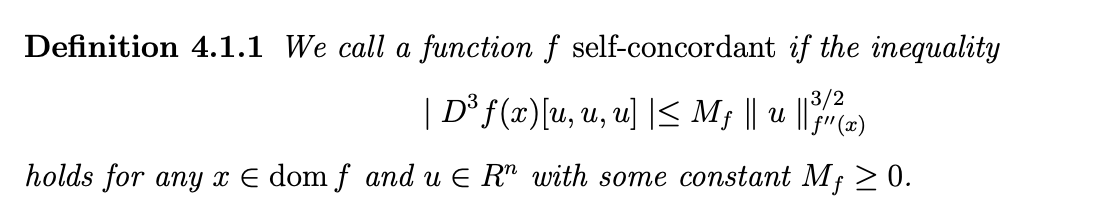
\includegraphics[width = 0.8\textwidth]{self_concordant_def.png}
% \end{figure}

\begin{tcolorbox}[bluebox, title = Self-concordant for univariate functions]
    A function $f: \mathbb{R} \to \mathbb{R}$ is self-concordant on $\mathbb{R}$ if :
    \begin{align*}
        |f'''(x)| \leq 2 f''(x)^{3/2}
    \end{align*}
\end{tcolorbox}

\begin{claim}
    \begin{align*}
        |\varphi'''(u)| \leq 2 \varphi''(u)^{3/2}
    \end{align*}
\end{claim}

\begin{claimproof}
    Let us define:

    \begin{align*}
        y_i := u + \nabla f(x_t)[i] + \frac{1}{x_t[i]}, \qquad \forall i = 1, \dots, d
    \end{align*}

    Then, the original function $\varphi(u)$ can be rewritten as:

    \begin{align*}
        \varphi(u) = u - \sum_{i=1}^d \log y_i = u + \sum_{i=1}^d (-\log y_i)
    \end{align*}

    Now we can compute the dirivatives of $\varphi(u)$:

    \begin{align*}
        \varphi'(u) = 1 - \sum_{i=1}^d \frac{1}{y_i}
    \end{align*}
    
    and the second derivative:

    \begin{align*}
        \varphi''(u) = \sum_{i=1}^d \frac{1}{y_i^2}
    \end{align*}

    and the third derivative:
    
    \begin{align*}
        \varphi'''(u) = -2 \sum_{i=1}^d \frac{1}{y_i^3}
    \end{align*}

    Now we have:
    
    \begin{align*}
        |\varphi'''(u)| &= 2 \sum_{i=1}^d \frac{1}{y_i^3} \\
        \varphi''(u) &= \sum_{i=1}^d \frac{1}{y_i^2} \\
    \end{align*}

    % Then we calculate $2\varphi''(u)^{3/2}$:

    % \begin{align*}
    %     2\varphi''(u)^{3/2} 
    %     &= 2 \left( \sum_{i=1}^d \frac{1}{y_i^2} \right)^{3/2} \\
    %     &=  \\
    % \end{align*}

    In order to let the original definition of $\varphi(u)$ be valid, $y_i \in (0, \infty)$ must hold, 
    thus, if we further define $g(y_i) = - \log y_i$, 
    then 
    
    \begin{align*}
        g : \{y_i \in \mathbb{R} \mid y_i > 0\} \rightarrow \mathbb{R}
    \end{align*}

    , and we have:

    \begin{align*}
        g'(y_i) &= \frac{d}{dy_i} (- \log y_i) = -\frac{1}{y_i} \\
        g''(y_i) &= \frac{d}{dy_i} \left( -\frac{1}{y_i} \right) = \frac{1}{y_i^2} \\
        g'''(y_i) &= \frac{d}{dy_i} \left( \frac{1}{y_i^2} \right) = -\frac{2}{y_i^3} \\
    \end{align*}

    And we have:

    \begin{align*}
        \mid g'''(y_i) \mid = \mid -\frac{2}{y_i^3} \mid = \frac{2}{y_i^3} \leq 2 \left( \frac{1}{y_i^2} \right)^{3/2} = 2 \left(\frac{1}{y_i^3} \right)
    \end{align*}

    Which shows that $g(y_i)$ is self-concordant.
    \bigskip

    Then, using the following property
    \footnote{G. Farina, \textit{Lecture 14A–B: Self-concordant functions}, MIT 6.7220/15.084 — Nonlinear Optimization, Apr.~16--18$^{\text{th}}$ 2024. Available at: \url{https://www.mit.edu/~gfarina/2024/67220s24_L14B_self_concordance/L14.pdf}, p.~4.}:

    \begin{figure}[H]
        \centering
        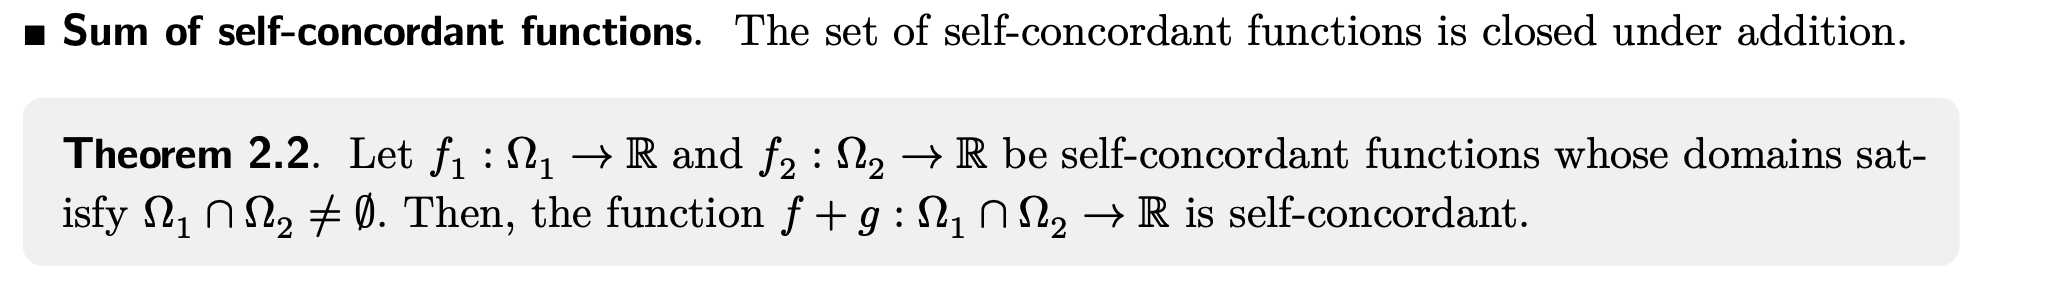
\includegraphics[width = 0.8\textwidth]{sum_self_concordant.png}
    \end{figure}

    Since $g(y_i)$ is self-concordant for all $i = 1, \dots, d$,
    and they have the same domain, so $\bigcap_{i = 1}^d \domain g(y_i) \neq \emptyset$,
    thus, their sum:

    \begin{align*}
        \sum_{i = 1}^d g(y_i) = \sum_{i = 1}^d (-\log y_i)
    \end{align*}

    is also self-concordant.

    \bigskip

    Then, using another property:

    \begin{figure}[H]
        \centering
        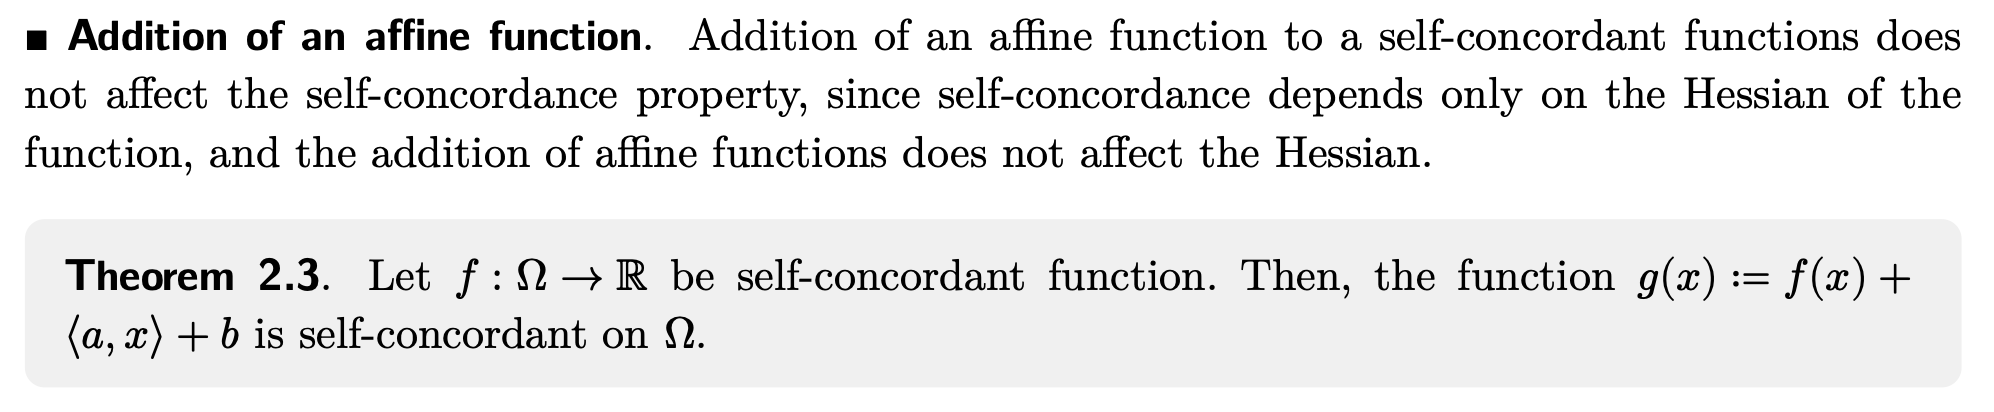
\includegraphics[width = 0.8\textwidth]{affine_self_concordant.png}
    \end{figure}

    If we let $h(u) = u$, then $h$ is an affine function, 
    then our self concordant function $\sum_{i = 1}^d (-\log y_i)$ plussing the affine function $h$:

    \begin{align*}
        \varphi(u) = u + \sum_{i = 1}^d (-\log y_i) 
    \end{align*}

    is also self-concordant.

\end{claimproof}
\end{solution}

% Considering the given condition for learning a linear classifier, with data:

% \begin{align*}
%     (x_1, y_1), \dots, (x_n, y_n) \in \mathbb{R}^d \times \{\pm 1\}
% \end{align*}

% , $l_1$-regularized lasso yields the following optimization problem:

% \begin{align*}
%     w_\star \in \arg\min_{w \in \mathbb{R}^d} f(w) + \lambda g(w), \quad \text{with} \ \lambda > 0
% \end{align*}


\section*{6}

We're given that:

\begin{align*}
    g_\mu(w) = \max_{v \in \mathcal{B}_\infty}\langle w, v \rangle - \frac{\mu}{2} \Vert v \Vert^2_2
\end{align*}

where $\mathcal{B}_\infty$ is the unit $l_\infty$ norm ball.
\bigskip

We need to show that $g_\mu$ is differentiable and:

\begin{align*}
    \nabla g_\mu(w) = 
    \begin{cases}
        1 \qquad &\text{if } w[i] \geq \mu \\
        \frac{w[i]}{\mu} \qquad &\text{if } - \mu \leq w[i] \leq \mu \\
        -1 \qquad &\text{if } w[i] < - \mu \\
    \end{cases}
\end{align*}

\begin{solution}
    % Since the dual of $l_\infty$ norm is $l_1$ norm, we have
    % \footnote{S. Boyd, \textit{Convex Optimization}, 1st ed., Cambridge University Press, Cambridge, UK, 2004, p.~637.}:
    % \begin{align*}
    %     \sup \{{w^Tv \mid \Vert v \Vert_\infty \leq 1}\} = \sum_{i = 1}^d \vert w[i] \vert = \Vert w \Vert_1
    % \end{align*}

    By the definition of $l_\infty$ norm, we have:

    \begin{align*}
        \Vert v \Vert_\infty \leq 1 \iff \max_{i = 1, \dots, d} \vert v[i] \vert \leq 1
    \end{align*}

    Then the original $g_\mu(w)$ can be rewritten as:

    \begin{align*}
        g_\mu(w) = \max_{v \in \mathcal{B}_\infty} \sum_{i=1}^d \left( w[i] v[i] - \frac{\mu}{2} v[i]^2\right), \qquad \text{where } \Vert v \Vert_\infty \leq 1
    \end{align*}

    Since to find the $v$ that maximizes the above expression, 
    we can independently find each $v[i]$ that maximizes the component in the summation, 
    so we can further define:

    \begin{align*}
        h_i(w[i]) = \max_{|v[i]| \leq 1} \left( w[i] v[i] - \frac{\mu}{2} v[i]^2 \right)
    \end{align*}

    Then the original $g_\mu(w)$ can be rewritten as:

    \begin{align*}
        g_\mu(w) = \sum_{i=1}^d h_i(w[i])
    \end{align*}

    Now we can prove the differentiability of $g_\mu(w)$ by proving the differentiability of each $h_i(w[i])$.
    Let:

    \begin{align*}
        f_{w[i]}(v[i]) = w[i] v[i] - \frac{\mu}{2} v[i]^2
    \end{align*}

    Since $w[i] v[i]$ is linear in $v[i]$, 
    and the quadratic term $-\frac{\mu}{2} v[i]^2 < 0 \ (\text{for } \mu > 0)$, 
    $f_{w[i]}(v[i])$ is concave in $v[i]$, 
    which means that exists a unique $v^\star[i]$ that maximizes $f_{w[i]}(v[i])$, 
    and we have:

    \begin{align*}
        \frac{d}{dv[i]} f_{w[i]}(v[i]) = w[i] - \mu v[i] = 0 \iff v[i]^* = \frac{w[i]}{\mu}
    \end{align*}

    Thus, if we do not restrict the solution to be in the unit ball, 
    the $v$ that maximizes $\langle w, v \rangle - \frac{\mu}{2} \Vert v \Vert^2_2$ is:

    \begin{align*}
        v^* 
        = \begin{bmatrix}
            \frac{w[1]}{\mu} \\
            \vdots \\
            \frac{w[d]}{\mu}
        \end{bmatrix}
        = \begin{bmatrix}
            v[1] \\
            \vdots \\
            v[d]
        \end{bmatrix}
    \end{align*}

    To further impose the restriction that $\max_{i = 1, \dots, d} \vert v[i] \vert \leq 1$, 
    the optimal $v$ need to satisfy:

    \begin{align*}
        v[i] \in [-1, 1]
    \end{align*}

    Thus, we need to project $v[i]$ to the interval $[-1, 1]$, 
    by the following definition of Euclidean projection
    \footnote{S. Boyd, \textit{Convex Optimization}, 1st ed., Cambridge University Press, Cambridge, UK, 2004, p.~399.}:

    \begin{figure}[H]
        \centering
        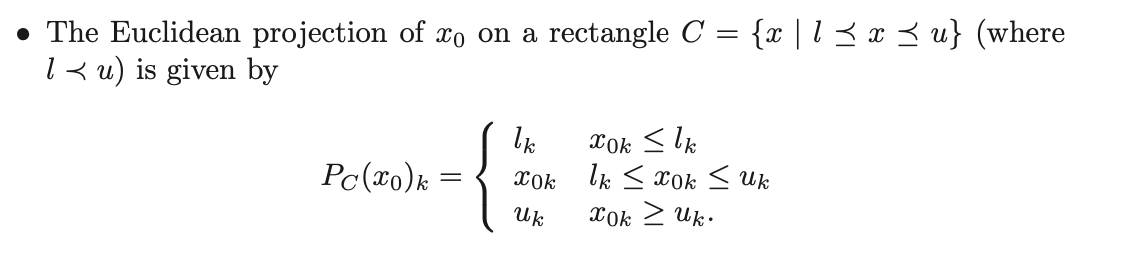
\includegraphics[width = 0.8\textwidth]{euclidean_projection.png}
    \end{figure}

    We have:

    \begin{align*}
        \text{proj}_{[-1, 1]}(v[i]) = \begin{cases}
            -1 \qquad &\text{if } v[i] < -1 \\
            v[i] \qquad &\text{if } -1 \leq v[i] \leq 1 \\
            1 \qquad &\text{if } v[i] > 1 \\
        \end{cases}
    \end{align*}

    or equivalently:

    \begin{align*}
        \text{proj}_{[-1, 1]}\left( \frac{w[i]}{\mu} \right) 
        = v^\star(w[i])
        = \begin{cases}
            -1 \qquad &\text{if } w[i] < - \mu \\
            \frac{w[i]}{\mu} \qquad &\text{if } \vert w[i]\vert \leq \mu \\
            1 \qquad &\text{if } w[i] > \mu \\
        \end{cases} \tag{1}
    \end{align*}

    And this matches the given $\nabla g_\mu(w)[i]$.
    \bigskip

    Then getting back to the part of proving differentiability, we have $h_i(w[i])$:

    \begin{align*}
        h_i(w[i]) 
        &= \max_{|v[i]| \leq 1} \left( w[i] v[i] - \frac{\mu}{2} v[i]^2 \right) \\
        &= \max_{|v[i]| \leq 1} \left(f_{w[i]}(v[i])\right) \\
        &= f_{w[i]}(v^\star(w[i])) \\
        &= w[i] v^\star (w[i]) - \frac{\mu}{2} (v^\star (w[i]))^2 \tag{2}
    \end{align*}

    Consider the three cases of $\text{proj}_{[-1, 1]}(v[i])$ in $(1)$:
    \bigskip

    \begin{itemize}
        \item \underline{Case 1:} $w[i] < - \mu$
        \bigskip

        Then $v^\star(w[i]) = -1$, and by plugging it into $(2)$:
        \begin{align*}
            &h_i(w[i]) = w[i] (-1) - \frac{\mu}{2} (-1)^2 = - w[i] - \frac{\mu}{2} \\
            \rightarrow \ & h_i'(w[i]) = \frac{d}{dw[i]} \left( - w[i] - \frac{\mu}{2} \right) = -1 \\
        \end{align*}

        \item \underline{Case 2:} $- \mu \leq w[i] \leq \mu$
        \bigskip

        Then $v^\star(w[i]) = \frac{w[i]}{\mu}$, and by plugging it into $(2)$:
        \begin{align*}
            &h_i(w[i]) = w[i] \frac{w[i]}{\mu} - \frac{\mu}{2} \left( \frac{w[i]}{\mu} \right)^2 = \frac{w[i]^2}{\mu} - \frac{\mu}{2} \frac{w[i]^2}{\mu^2} = \frac{w[i]^2}{2\mu} \\
            \rightarrow \ & h_i'(w[i]) = \frac{d}{dw[i]} \left( \frac{w[i]^2}{2\mu} \right) = \frac{w[i]}{\mu} \\
        \end{align*}

        \item \underline{Case 3:} $w[i] > \mu$
        \bigskip

        Then $v^\star(w[i]) = 1$, and by plugging it into $(2)$:
        \begin{align*}
            &h_i(w[i]) = w[i] (1) - \frac{\mu}{2} (1)^2 = w[i] - \frac{\mu}{2} \\
            \rightarrow \ & h_i'(w[i]) = \frac{d}{dw[i]} \left( w[i] - \frac{\mu}{2} \right) = 1 \\
        \end{align*}
    \end{itemize}

    Thus, at the boundaries:

    \begin{itemize}
        \item $w[i] = \mu$
        \bigskip

        Left derivative:
        \begin{align*}
            \lim_{w[i] \to \mu^-} h_i'(w[i]) = \lim_{w[i] \to \mu^-} \frac{w[i]}{\mu} = \frac{\mu}{\mu} = 1
        \end{align*}

        Right derivative:
        \begin{align*}
            \lim_{w[i] \to \mu^+} h_i'(w[i]) = 1
        \end{align*}

        \item $w[i] = - \mu$
        \bigskip

        Left derivative:
        \begin{align*}
            \lim_{w[i] \to - \mu^-} h_i'(w[i]) = -1
        \end{align*}

        Right derivative:
        \begin{align*}
            \lim_{w[i] \to - \mu^+} h_i'(w[i]) = \lim_{w[i] \to - \mu^+} \frac{w[i]}{\mu} = \frac{- \mu}{\mu} = -1
        \end{align*}
    \end{itemize}

    And in the interior:

    \begin{align*}
        h_i'(w[i]) 
        &= w[i] \frac{w[i]}{\mu} - \frac{\mu}{2} \left(\frac{w[i]}{\mu}\right)^2 \\
        &= \frac{w[i]^2}{\mu} - \frac{w[i]^2}{2\mu} \\
        &= \frac{w[i]^2}{2\mu}
    \end{align*}

    Which always exists and is unique.
    \bigskip

    Therefore, $h_i(w[i])$ is differentiable, and $g_\mu(w) = \sum_{i=1}^d h_i(w[i])$ is a sum of differentiable functions, 
    so $g_\mu(w)$ is also differentiable.
    
\end{solution}

\section*{7}

We need to further prove that $g_\mu$ is $\frac{1}{\mu}$-smooth.

\begin{solution}

    By the definition in the following image
    \footnote{A. Sidford, \textit{MS\&E 213 / CS 269O: Chapter 2 — Smooth Functions}, Stanford University, Oct.~17, 2020. Available at: \url{https://web.stanford.edu/~sidford/courses/20fa_opt_theory/sidford_mse213_2020fa_chap_2_smoothness.pdf}, p.~2.}:

    \begin{figure}[H]
        \centering
        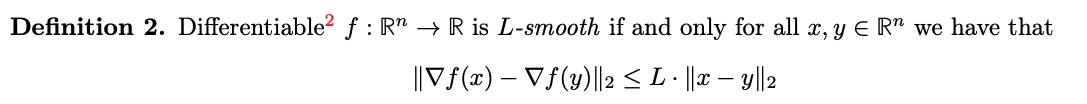
\includegraphics[width = 0.8\textwidth]{L_smooth_def.png}
    \end{figure}

    % \footnote{Lecture 4: Mirror Descent, p.~10}, we have:

    % \begin{tcolorbox}[bluebox, title = $L$-Smooth]
    %     We say a differentiable function $f: \mathbb{R}^d \to \mathbb{R}$ is $L$-smooth for some $L > 0$ if:

    %     \begin{align*}
    %         f(y) \leq f(x) + \langle \nabla f(x), y - x \rangle + \frac{L}{2} \Vert y - x \Vert_2^2, \qquad \forall x, y \in \mathbb{R}^d
    %     \end{align*}
    % \end{tcolorbox}

    Since we have already proved that $g_\mu(w)$ is differentiable, 
    proving the following claim is equivalent to proving that $g_\mu(w)$ is $\frac{1}{\mu}$-smooth.

    \bigskip

    \begin{claim}
        \begin{align*}
            \Vert \nabla g_\mu(w_1) - \nabla g_\mu(w_2) \Vert_2 \leq \frac{1}{\mu} \Vert w_1 - w_2 \Vert_2, \qquad \forall w_1, w_2 \in \mathbb{R}^d
        \end{align*}
    \end{claim}

    \begin{claimproof}
        Following the notation in the previous subproblem, we have:
        
        \begin{align*}
            \nabla g_\mu(w) = \begin{bmatrix}
                \nabla g_\mu(w)[1] \\
                \vdots \\
                \nabla g_\mu(w)[d]
            \end{bmatrix}
        \end{align*}

        Let:

        \begin{align*}
            w_1 = \begin{bmatrix}
                w_1[1] \\
                \vdots \\
                w_1[d]
            \end{bmatrix}, \quad w_2 = \begin{bmatrix}
                w_2[1] \\
                \vdots \\
                w_2[d]
            \end{bmatrix}
        \end{align*}

        Then we have:

        \begin{align*}
            \nabla g_\mu(w_1) - \nabla g_\mu(w_2) 
            = \begin{bmatrix}
                \nabla g_\mu(w_1)[1] - \nabla g_\mu(w_2)[1] \\
                \vdots \\
                \nabla g_\mu(w_1)[d] - \nabla g_\mu(w_2)[d]
            \end{bmatrix}
        \end{align*}

        The maximum of $\Vert \nabla g_\mu(w_1) - \nabla g_\mu(w_2) \Vert_2$ happens when:

        \begin{align*}
            \nabla g_\mu(w_1) = \begin{bmatrix}
                1 \\
                \vdots \\
                1
            \end{bmatrix}
            \quad \text{and} \quad
            \nabla g_\mu(w_2) = \begin{bmatrix}
                -1 \\
                \vdots \\
                -1
            \end{bmatrix}
        \end{align*}

        which implies that:

        \begin{align*}
            w_1[i] \geq \mu, \ w_2[i] \leq - \mu \qquad \forall i = 1, \dots, d \tag{1}
        \end{align*}

        and we'll have:

        \begin{align*}
            \Vert \nabla g_\mu(w_1) - \nabla g_\mu(w_2) \Vert_2 
            = \Vert \begin{bmatrix}
                1 \\
                \vdots \\
                1
            \end{bmatrix} - \begin{bmatrix}
                -1 \\
                \vdots \\
                -1
            \end{bmatrix} \Vert_2
            = 2 \sqrt{d}
        \end{align*}

        Under the condition in $(1)$, if we want to find the minimium of $L \Vert w_1 - w_2 \Vert_2$, 
        we can set $w_1[i] = \mu$ and $w_2[i] = - \mu$ for all $i = 1, \dots, d$, 
        and we'll have:

        \begin{align*}
            L \Vert w_1 - w_2 \Vert_2 = L \Vert \begin{bmatrix}
                \mu \\
                \vdots \\
                \mu
            \end{bmatrix} - \begin{bmatrix}
                - \mu \\
                \vdots \\
                - \mu
            \end{bmatrix} \Vert_2 = L \sqrt{4 \mu^2 d} = L 2 \mu \sqrt{d}
        \end{align*}

        Thus, we can set $L = \frac{1}{\mu}$, and we'll have:

        \begin{align*}
            \Vert \nabla g_\mu(w_1) - \nabla g_\mu(w_2) \Vert_2 = 2 \sqrt{d} \leq 2 \sqrt{d} = \frac{1}{\mu} 2 \mu \sqrt{d} = \frac{1}{\mu} \Vert w_1 - w_2 \Vert_2 
        \end{align*}
    \end{claimproof}
\end{solution}

\section*{8}

We're asked to show that:

\begin{align*}
    g_\mu(w) \leq g(w) \leq g_\mu(w) + \frac{\mu d}{2} 
\end{align*}

\begin{solution}

    Since $g(w)$ is defined as $\Vert w \Vert_1$, it is equivalent to show that:

    \begin{align*}
        g_\mu(w) \leq \Vert w \Vert_1  = \sum_{i=1}^d \vert w[i] \vert \leq g_\mu(w) + \frac{\mu d}{2} 
    \end{align*} 

    We prove this by showing the two inequalities separately.

    \begin{itemize}
        \item \underline{$g_\mu(w) \leq g(w)$} 
        \bigskip

        Since the dual norm of $\Vert \cdot \Vert_1$ is $\Vert \cdot \Vert_\infty$, 
        we can rewrite the one norm $\Vert w \Vert_1$ as
        \footnote{S. Boyd, \textit{Convex Optimization}, 1st ed., Cambridge University Press, Cambridge, UK, 2004, p.~637.}:

        \begin{align*}
            g(w) = \Vert w \Vert_1 = \sup \{w^T v \mid \Vert v \Vert_\infty \leq 1\}
        \end{align*}
        
        Compared with the definition of $g_\mu(w)$, we have:

        \begin{align*}
            g_\mu(w) = \max_{v \in \mathcal{B}_\infty} \langle w, v \rangle - \frac{\mu}{2} \Vert v \Vert_2^2
        \end{align*}

        Since $\mu$ is positive, and the square of a two norm $\Vert v \Vert_2^2$ is always non-negative, 
        the term $\frac{\mu}{2} \Vert v \Vert_2^2$ is always non-negative, thus:

        \begin{align*}
            g_\mu(w) = \max_{v \in \mathcal{B}_\infty} \langle w, v \rangle - \frac{\mu}{2} \Vert v \Vert_2^2 
            \leq \sup \{w^T v \mid \Vert v \Vert_\infty \leq 1\} = g(w)
        \end{align*}

        \item \underline{$g(w) \leq g_\mu(w) + \frac{\mu d}{2}$}
        \bigskip

        Observe that:

        \begin{align*}
            g(w)
            = \Vert w \Vert_1 
            = \sum_{i=1}^d \vert w[i] \vert 
            = \left[ w[1] \cdots w[d] \right] 
            \begin{bmatrix}
                \mathrm{sign}(w[1]) \\
                \vdots \\
                \mathrm{sign}(w[d])
            \end{bmatrix}
            = \langle w, \mathrm{sign}(w) \rangle
        \end{align*}

        where $\mathrm{sign}(w)$ is the sign function, which is defined as:
        
        \begin{align*}
            \mathrm{sign}(w[i]) = \begin{cases}
                1 \qquad &\text{if } w[i] > 0 \\
                -1 \qquad &\text{if } w[i] \leq 0 \\
            \end{cases}
        \end{align*}

        Then let:

        \begin{align*}
            v^\star = \arg\max_{v \in \mathcal{B}_\infty} \langle w, v \rangle = \mathrm{sign}(w)
        \end{align*}

        Since for all elements in $\mathrm{sign}(w)$, its value is either $1$ or $-1$, 
        $\mathrm{sign}(w) \in \mathcal{B}_\infty$.

        Thus, we can write:

        \begin{align*}
            g_\mu(w) 
            &= \langle w, \mathrm{sign}(w) \rangle - \frac{\mu}{2} \Vert \mathrm{sign}(w) \Vert_2^2 \\
            &= g(w) - \frac{\mu}{2} \cdot d \\
        \end{align*}

        And we can get the following inequality:

        \begin{align*}
            g_\mu(w) 
            &= \max_{v \in \mathcal{B}_\infty} \langle w, v \rangle - \frac{\mu}{2} \Vert v \Vert_2^2 \\
            &\geq \langle w, v^\star \rangle - \frac{\mu}{2} \Vert v^\star \Vert_2^2 \\
            &= g(w) - \frac{\mu}{2} d \\
        \end{align*}

        Therefore:

        \begin{align*}
            & g_\mu(w) \geq g(w) - \frac{\mu}{2} d \\
            \rightarrow \ & g(w) \leq g_\mu(w) + \frac{\mu d}{2}
        \end{align*}
    \end{itemize}
\end{solution}

\section*{9}

\begin{solution}

    We're given:

    \begin{align*}
        F = f + \lambda g
    \end{align*}

    \begin{claim}
        \begin{align*}
            F(w_{T+1}) - F(w_\star) 
            \leq 
            \frac{\lambda \sqrt{d}}{2 \sqrt{T}} \left( \| w_1 - w_\star \|_2^2 + 1 \right) + \frac{ L \|w_1 - w_\star\|_2^2}{2T}
        \end{align*}
    \end{claim}

    \begin{claimproof}
        \bigskip

        Let us define:

        \begin{align*}
            F_\mu(w) = f(w) + \lambda g_\mu(w)
        \end{align*}

        which is a little bit different from the original $F$ in the problem statement by replacing $g_\mu(w)$ with $g(w)$.
        \bigskip

        In the solution process, I aimed to use the following theorem
        \footnote{Lecture 6 of \textit{10-725: Optimization}, taught by Ryan Tibshirani at Carnegie Mellon University in Fall 2013. Scribed by Micol Marchetti-Bowick. URL: \url{https://www.stat.cmu.edu/~ryantibs/convexopt-F13/scribes/lec6.pdf}, p.~6-1}:

        \begin{figure}[H]
            \centering
            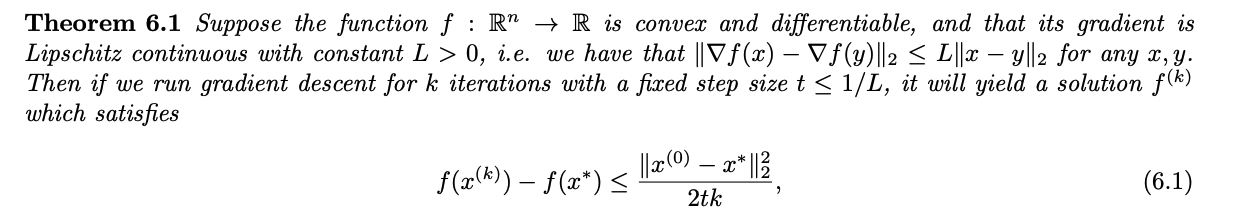
\includegraphics[width = 0.8\textwidth]{gradient_descent_convergence.png}
        \end{figure}

        Thus we need to prove the differentiability, convexity, and smoothness of $F_\mu(w)$.
        \bigskip

        \underline{$F_\mu(w)$ differentiable:}
        \bigskip

        We're given that $f$ is differentiable, and in the previous problem $6$, we have proved that $g_\mu(w)$ is differentiable, 
        thus $F_\mu(w)$ is differentiable.
        \bigskip

        \underline{$F_\mu(w)$ convex:}
        \bigskip

        We're given that $f$ is convex, so it remained to show that $g_\mu(w)$ is convex.

        \begin{align*}
            g_\mu(w) = \max_{v \in \mathcal{B}_\infty} \langle w, v \rangle - \frac{\mu}{2} \Vert v \Vert_2^2
        \end{align*}

        Since $\langle w, v \rangle - \frac{\mu}{2} \Vert v \Vert_2^2$ is affine, it is convex, 
        and taking the maximum of a convex function is convex, thus $g_\mu(w)$ is convex.
        \bigskip

        With both $f$ and $g_\mu(w)$ being convex, 
        and the operations of addition and multiplication by a constant preserve convexity, 
        $F_\mu(w)$ is convex.
        \bigskip

        \underline{$F_\mu(w)$ smooth:}
        \bigskip

        We're given that $f$ is $L$-smooth, 
        and in the previous problem $7$, we have proved that $g_\mu(w)$ is $\frac{1}{\mu}$-smooth, 
        thus by the definition of $L$-smoothness
        \footnote{A. Sidford, \textit{MS\&E 213 / CS 269O: Chapter 2 — Smooth Functions}, Stanford University, Oct.~17, 2020. Available at: \url{https://web.stanford.edu/~sidford/courses/20fa_opt_theory/sidford_mse213_2020fa_chap_2_smoothness.pdf}, p.~2.}:

        \begin{figure}[H]
            \centering
            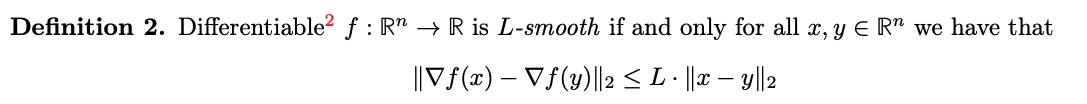
\includegraphics[width = 0.8\textwidth]{L_smooth_def.png}
        \end{figure}

        % thus by the following lemma
        % \footnote{Reza Zadeh, *CME 323: Distributed Algorithms and Optimization, Spring 2020*, Lecture 8, 
        % scribed by Andreas Santucci, edited by Robin Brown, Stanford University, Apr. 23, 2020. 
        % Available at: \url{https://stanford.edu/~rezab/dao/notes/L08/cme323_lec8.pdf}, p.~4.}:
        
        % \begin{figure}[H]
        %     \centering
        %     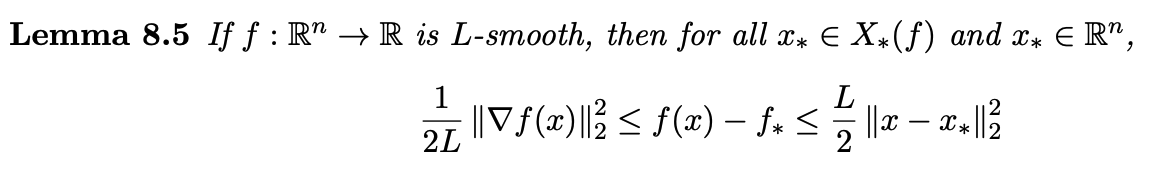
\includegraphics[width = 0.8\textwidth]{L_smooth_bound.png}
        % \end{figure}
        
        % we have:

        % \begin{align*}
        %     g_\mu(w_{T+1}) - g_\mu(w_\star) 
        %     \leq 
        %     \frac{1}{2\mu} \Vert w_{T+1} - w_\star \Vert_2^2
        % \end{align*}

        we have:

        \begin{align*}
            \Vert \nabla f(w_1) - \nabla f(w_2) \Vert_2 &\leq L \Vert w_1 - w_2 \Vert_2 \\ 
            \Vert \nabla g_\mu(w_1) - \nabla g_\mu(w_2) \Vert_2 &\leq \frac{1}{\mu} \Vert w_1 - w_2 \Vert_2 \tag{1}
        \end{align*}

        We then take gradient to the definition of $F_\mu(w)$:

        \begin{align*}
            \nabla F_\mu(w) = \nabla f(w) + \lambda \nabla g_\mu(w)
        \end{align*}

        with triangle inequality, and replace $(1)$ in, we have:

        \begin{align*}
            \Vert \nabla F_\mu(w_1) - \nabla F_\mu(w_2) \Vert_2 
            &= \Vert \nabla f(w_1) + \lambda \nabla g_\mu(w_1) - \nabla f(w_2) - \lambda \nabla g_\mu(w_2) \Vert_2 \\
            &= \Vert \nabla f(w_1) - \nabla f(w_2) + \lambda \nabla g_\mu(w_1) - \lambda \nabla g_\mu(w_2) \Vert_2 \\
            &\leq \Vert \nabla f(w_1) - \nabla f(w_2) \Vert_2 + \lambda \Vert \nabla g_\mu(w_1) - \nabla g_\mu(w_2) \Vert_2 \\
            &\leq L \Vert w_1 - w_2 \Vert_2 + \frac{\lambda}{\mu} \Vert w_1 - w_2 \Vert_2 \\
            &= \left(L + \frac{\lambda}{\mu}\right) \Vert w_1 - w_2 \Vert_2
        \end{align*}

        Thus we have derived that $F_\mu(w)$ is $L + \frac{\lambda}{\mu}$-smooth.
        \bigskip

        Thus we can use the theorem above and get:

        \begin{align*}
            F_\mu(w_{T+1}) - F_\mu(w_\star) 
            &\leq \frac{\left(L + \frac{\lambda}{\mu}\right) \Vert w_1 - w_\star \Vert^2_2}{2T} \\
            % &= \frac{\left(\frac{\lambda}{\mu}\right) \Vert w_1 - w_\star \Vert^2_2}{2T} + \frac{L \Vert w_1 - w_\star \Vert^2_2}{2T} \\
        \end{align*}

        From problem $8$, we have proved that:

        \begin{align*}
            g_\mu(w) \leq g(w) \leq g_\mu(w) + \frac{\mu d}{2}
        \end{align*}

        so we have:

        \begin{align*}
            g(w_{T+1}) &\leq g_\mu(w_{T+1}) + \frac{\mu d}{2} \\
            g_\mu(w_\star) &\leq g(w_\star) \qquad (\text{or } -g(w_\star) \leq -g_\mu(w_\star))
        \end{align*}

        and we could finally derive:

        \begin{align*}
            F(w_{T+1}) - F(w_\star) 
            &= f(w_{T+1}) + \lambda \textcolor{blue}{g(w_{T+1})} - f(w_\star) - \lambda \textcolor{blue}{g(w_\star)} \\
            &\leq f(w_{T+1}) + \lambda \textcolor{blue}{\left(g_\mu(w_{T+1}) + \frac{\mu d}{2}\right)} - f(w_\star) - \lambda \textcolor{blue}{\left(g_\mu(w_\star)\right)} \\
            &= \textcolor{Green}{f(w_{T+1}) + \lambda \left(g_\mu(w_{T+1})\right)} + \frac{\lambda \mu d}{2} \textcolor{Green}{- f(w_\star) - \lambda \left(g_\mu(w_\star)\right)} \\
            &= \textcolor{Green}{F_\mu(w_{T+1}) - F_\mu(w_\star) } + \frac{\lambda \mu d}{2} \\
            &\leq \frac{\left(L + \frac{\lambda}{\mu}\right) \Vert w_1 - w_\star \Vert^2_2}{2T} + \frac{\lambda \mu d}{2} \\
            &= \frac{L \Vert w_1 - w_\star \Vert^2_2}{2T} + \frac{\frac{\lambda}{\mu} \Vert w_1 - w_\star \Vert^2_2}{2T} + \frac{\lambda \mu d}{2} \\
            &= \frac{L \Vert w_1 - w_\star \Vert^2_2}{2T} + \frac{\lambda \left( \frac{1}{\mu} \Vert w_1 - w_\star \Vert^2_2 + T \mu d \right)}{2T} \tag{*}
        \end{align*}

        By setting $\mu = \frac{1}{\sqrt{Td}}$, we have:

        \begin{align*}
            F(w_{T+1}) - F(w_\star) 
            &\leq \frac{L \Vert w_1 - w_\star \Vert^2_2}{2T} + \frac{\lambda \left( \frac{1}{\mu} \Vert w_1 - w_\star \Vert^2_2 + T \mu d \right)}{2T} \\
            &= \frac{L \Vert w_1 - w_\star \Vert^2_2}{2T} + \frac{\lambda \left( \sqrt{Td} \Vert w_1 - w_\star \Vert^2_2 + T \frac{1}{\sqrt{Td}} d \right)}{2T} \\
            &= \frac{L \Vert w_1 - w_\star \Vert^2_2}{2T} + \frac{\lambda \left( \sqrt{Td} \Vert w_1 - w_\star \Vert^2_2 + \sqrt{Td} \right)}{2T} \\
            &= \frac{L \Vert w_1 - w_\star \Vert^2_2}{2T} + \frac{\lambda \sqrt{Td} \left( \Vert w_1 - w_\star \Vert^2_2 + 1 \right)}{2T} \\
            &= \frac{L \Vert w_1 - w_\star \Vert^2_2}{2T} + \frac{\lambda \sqrt{d} \left( \Vert w_1 - w_\star \Vert^2_2 + 1 \right)}{2\sqrt{T}} \\
        \end{align*}
        
        Which is the required bound.
    \end{claimproof}
\end{solution}

\section*{10}

\begin{solution}
    % we should take the derivative w.r.t. $\mu$ and set it to $0$ to get the optimal $\mu$:
    
% \begin{align*}
%     &\frac{d}{d\mu} \left( \frac{\left(L + \frac{\lambda}{\mu}\right) \Vert w_1 - w_\star \Vert^2_2}{2T} + \frac{\lambda \mu d}{2} \right) = 0 \\
%     \rightarrow \ & \frac{\left(-\lambda\right) \Vert w_1 - w_\star \Vert^2_2}{2T\mu^2} + \frac{\lambda d}{2} = 0 \\
%     \rightarrow \ & \frac{\lambda d}{2} = \frac{\lambda \Vert w_1 - w_\star \Vert^2_2}{2T\mu^2} \\
%     \rightarrow \ & d = \frac{\Vert w_1 - w_\star \Vert^2_2}{T\mu^2} \\
%     \rightarrow \ & \mu^2 = \frac{\Vert w_1 - w_\star \Vert^2_2}{Td} \\
%     \rightarrow \ & \mu = \sqrt{\frac{\Vert w_1 - w_\star \Vert^2_2}{Td}} \\
%     \rightarrow \ & \mu = \sqrt{\frac{\Vert w_1 - w_\star \Vert^2_2}{Td}}
% \end{align*}

% Substitute $\mu = \sqrt{\frac{\Vert w_1 - w_\star \Vert^2_2}{Td}}$ into $(*)$, we have:

% \begin{align*}
%     F(w_{T+1}) - F(w_\star) 
%     &\leq \frac{L \Vert w_1 - w_\star \Vert^2_2}{2T} + \frac{\lambda \left( \frac{1}{\mu} \Vert w_1 - w_\star \Vert^2_2 + T \mu d \right)}{2T} \\
%     &= \frac{L \Vert w_1 - w_\star \Vert^2_2}{2T} + \frac{\lambda \left( \frac{1}{\sqrt{\frac{\Vert w_1 - w_\star \Vert^2_2}{Td}}} \Vert w_1 - w_\star \Vert^2_2 + T \sqrt{\frac{\Vert w_1 - w_\star \Vert^2_2}{Td}} d \right)}{2T} \\
% \end{align*}

    We want to get a tighter bound using accelerated gradient descent and choose other value of $\mu$. 
    By the following theorem
    \footnote{Sébastien Bubeck. \textit{Convex Optimization: Algorithms and Complexity}. 
    Foundations and Trends\textsuperscript{\textregistered} in Machine Learning, Vol. 8, No. 3-4 (2015), pp. 231–357. Page 294. 
    DOI: 10.1561/2200000050. Available at: \url{http://sbubeck.com/Bubeck15.pdf}}:

    \begin{figure}[H]
        \centering
        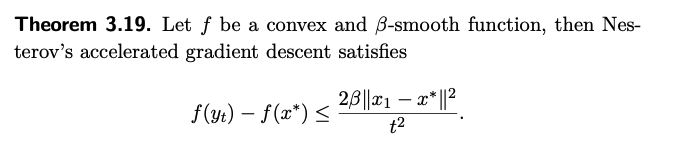
\includegraphics[width = 0.8\textwidth]{NAG.png}
    \end{figure}

    Since we derived that our $F_\mu(w)$ is $L + \frac{\lambda}{\mu}$-smooth in the previous problem $9$, 
    we have the following inequality:

    \begin{align*}
        F_\mu(w_{T+1}) - F_\mu(w_\star) 
        &\leq \frac{ 2 \left(L + \frac{\lambda}{\mu}\right) \Vert w_1 - w_\star \Vert^2_2}{T^2} \\
    \end{align*}

    Using the same process as in problem $9$ 
    (please refer to the last part, especially the part with tag $(*)$ if needed)
    , we derive the bound on $F(w_{T+1}) - F(w_\star)$:

    \begin{align*}
        F(w_{T+1}) - F(w_\star) 
        &\leq \frac{ 2 \left(L + \frac{\lambda}{\mu}\right) \Vert w_1 - w_\star \Vert^2_2}{T^2} + \frac{\lambda \mu d}{2} \\
    \end{align*}

    To show the improved optimization error bound, 
    we should take the derivative w.r.t. $\mu$ and set it to $0$ to get the optimal minimum value of the righthand side:

    \begin{align*}
        &\frac{d}{d\mu} \left( \frac{ 2 \left(L + \frac{\lambda}{\mu}\right) \Vert w_1 - w_\star \Vert^2_2}{T^2} + \frac{\lambda \mu d}{2} \right) = 0 \\
        \rightarrow \ & \frac{2 \lambda \Vert w_1 - w_\star \Vert^2_2}{T^2} \frac{d}{d\mu} \left( \frac{1}{\mu} \right) = - \frac{\lambda d}{2} \\
        \rightarrow \ & \frac{2 \lambda \Vert w_1 - w_\star \Vert^2_2}{T^2 \mu^2} = \frac{\lambda d}{2} \\
        \rightarrow \ & \frac{4 \Vert w_1 - w_\star \Vert^2_2}{d T^2 } = \mu^2 \\
        \rightarrow \ & \mu = \frac{2 \Vert w_1 - w_\star \Vert_2}{\sqrt{d} T} \\
    \end{align*}

    Substitute $\mu = \frac{2 \Vert w_1 - w_\star \Vert_2}{\sqrt{d} T}$ into the bound on $F(w_{T+1}) - F(w_\star)$, we have:

    \begin{align*}
        F(w_{T+1}) - F(w_\star) 
        &\leq \frac{ 2 \left(L + \frac{\lambda \sqrt{d} T}{2 \Vert w_1 - w_\star \Vert_2}\right) \Vert w_1 - w_\star \Vert^2_2}{T^2} 
        + \frac{\lambda d 2 \Vert w_1 - w_\star \Vert_2}{2\sqrt{d} T} \\
        &= \frac{2 L \Vert w_1 - w_\star \Vert^2_2}{T^2} 
        + \frac{\frac{\lambda \sqrt{d} T}{\Vert w_1 - w_\star \Vert_2} \Vert w_1 - w_\star \Vert_2^2}{T^2} 
        + \frac{\lambda \sqrt{d} \Vert w_1 - w_\star \Vert_2}{T} \\
        &= \frac{2 L \Vert w_1 - w_\star \Vert^2_2}{T^2} 
        + \frac{\lambda \sqrt{d} \Vert w_1 - w_\star \Vert_2^2}{T}
        + \frac{\lambda \sqrt{d} \Vert w_1 - w_\star \Vert_2}{T} \\
        &= \frac{2 L \Vert w_1 - w_\star \Vert^2_2}{T^2} 
        + \frac{\lambda \sqrt{d} \Vert w_1 - w_\star \Vert_2 (\Vert w_1 - w_\star \Vert_2 + 1)}{T}
    \end{align*}
\end{solution}

\section*{11}

\begin{solution}
    The rate of convergence of FISTA is shown as in the following image
    \footnote{Sébastien Bubeck. \textit{Convex Optimization: Algorithms and Complexity}. Page 311.}:

    \begin{figure}[H]
        \centering
        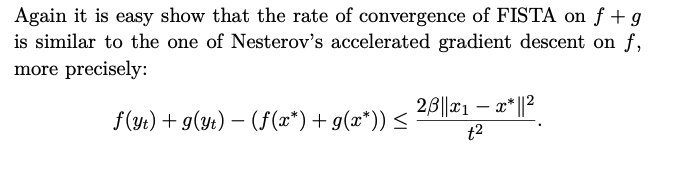
\includegraphics[width = 0.8\textwidth]{FISTA.png}
    \end{figure}

    This means that the rate of convergence of FISTA is $O\left(\frac{1}{T^2}\right)$, 
    however, in the previous problem $10$, we have proved that the rate of convergence of NAG is $O\left(\frac{1}{T}\right)$.

    Therefore, regarding the rate of convergence, FISTA is better than NAG.
    \bigskip
    
    In addition, from the resulting optimization error bound, 
    we can see that there is $\sqrt{d}$ in the bound of NAG, 
    which means that as the dimension $d$ increases, the performance to approximate $w_\star$ by $w_{T+1}$ will be worse.
\end{solution}
\end{document}